%------------------------------------------------------
%Author             : Jonathan Schwarz
%University         : Pforzheim University
%Date of last edit  : Fri, 06 Mar 2015 10:00:53 +0100
%Filename           : neural_networks.tex
%------------------------------------------------------

\documentclass[10pt,a4paper,DIV=11]{scrreprt}

%British English
\usepackage[UKenglish]{babel}
%utf8
\usepackage[utf8]{inputenc}

%pseudo-code
\usepackage[boxruled,vlined]{algorithm2e}

%for source code listings
\usepackage{listings}

\usepackage[table]{xcolor}

%tikz
\usepackage{tikz}
\usetikzlibrary{arrows,positioning,fit}

%plots
\usepackage{pgfplots}

%blocks - used by tikz-uml, included before
\pgfdeclarelayer{background}
\pgfdeclarelayer{foreground}
\pgfsetlayers{background,main,foreground}

%<,> in tikz-uml
\usepackage[T1]{fontenc}
\usepackage{tikz-uml}

%subfigure
\usepackage{graphicx}
\usepackage{subfigure}

%prevent figure from floating pictures
\usepackage{float}

%footer & header
\usepackage{fancyhdr}

%push footer down
\usepackage[bottom]{footmisc}

%footer & header
\pagestyle{fancy}
%clean footer & header
\fancyhf{}

%acronyms
\usepackage[nohyperlinks]{acronym}

%bibtex
\usepackage[square,numbers]{natbib}
\usepackage{gensymb}

%maths
\usepackage[tbtags]{amsmath}
\usepackage{amssymb} 
\usepackage{dsfont}

%japanese
\usepackage{CJKutf8}

%table of contents with hyperlinks
%always include as last package
\usepackage{hyperref}

%===========================TITLE PAGE=======================================

%university logo
\titlehead
{
    
\includegraphics[width=0.20\textwidth]{files/hspflogo.pdf}\\

    Pforzheim University\\
    School of Engineering\\
}

\subject{Project work}
	
\title
{
     A comparison of neural network types and learning techniques with an application in STOCA\cite{DANIEL}.
}

\author
{
    \textbf{Jonathan Schwarz} - matriculation number: 304727
}
\date
{
    Summer term 2015
}
%\today{}}

\publishers
{
    Examiner: Prof Dr Richard Alznauer\\
    Supervisor: Dr Christoph Ußfeller
}


%=========================================GLOBAL SETTINGS=========================================

%footer &header

%\fancyfoot[L]{\textbf{Multi-Threading mit POSIX-pThreads}}
\fancyhead[R]{Page \thepage}
%\fancyhead[L]{\thechapter}

%chapter number and title
\fancyhead[L]{\nouppercase{\leftmark}}
%line
%\renewcommand{\footrulewidth}{0.5 pt}
\usepackage{lmodern}
\addtokomafont{sectioning}{\rmfamily}
\setlength{\parindent}{0mm}

%colour definitions
\definecolor{dkgreen}{rgb}{0,0.6,0}
\definecolor{grey}{rgb}{0.7,0.7,0.7}
%medium grey
\definecolor{mgrey}{gray}{0.80}
%light grey
\definecolor{lgrey}{gray}{0.97}

%hyperlink settings
%frame around hyperlinks
\hypersetup
{
    colorlinks = false,
    linkcolor = black,
    hypertexnames = false,
    citecolor = green
}

%listing settings
\lstset
{ 
    language=C,                
    basicstyle=\footnotesize\ttfamily,           
    numbers=left,
    stepnumber=5,    
    firstnumber=1,
    numberfirstline=true                 
    numberstyle=\color{black},                 
    numbersep=5pt,                 
    backgroundcolor=\color{white},      
    showspaces=false,             
    showstringspaces=false,         
    showtabs=false,                
    frame=single,                   
    rulecolor=\color{black},       
    tabsize=2,                     
    captionpos=b,                   
    breaklines=true,                
    breakatwhitespace=false,       
    title=\lstname,                    
    keywordstyle=\color{blue},          
    commentstyle=\color{dkgreen}, 
    identifierstyle=\color{black},      
    stringstyle=\color{purple},      
    escapeinside={\%*}{*)},      
    morekeywords={*,...},            
    deletekeywords={...}             
}

\newenvironment{Japanese}{%
    \CJKfamily{min}%
    \CJKtilde
\CJKnospace}{}

\setcounter{tocdepth}{4}  %a deeper contents menue
%=====================================DOCUMENT START=========================
\begin{document}

\tikzstyle{line}=[draw]
\tikzstyle{arrow}=[draw, -latex] 

%\renewcommand*\contentsname{Content}
%\renewcommand*\listtablename{Tables}
%\renewcommand*\listfigurename{Figures}
%\renewcommand*\bibname{Literature references}

\maketitle
\thispagestyle{empty}
\newpage
{\large\tableofcontents}
\newpage

\thispagestyle{empty}

\section*{List of acronyms}
\begin{acronym}
    \acro{$ANN$}{Artificial neural network}
    \acro{$a_j$}{Activity of unit $n_j$}
    \acro{$a_j(t)$}{Activity of unit $n_j$ at time $t$}
    \acro{$H$}{The set of hidden layers of a neural network}
    \acro{$L$}{The set of layers of a neural network}
    \acro{$ML$}{Machine learning}
    \acro{$n_j$}{Neuron (also unit) $j$}
    \acro{$W$}{The connection matrix}
    \acro{$w_{ij}$}{Weight on the connection link between neuros $n_i$ and $n_j$}
%    \acro{$\Delta w_{ij}$}{Weight change  on the connection link between unit $i$ and $j$}
%    \acro{$\overrightarrow{x}$}{The input vector of a neural network}
%    \acro{$\overrightarrow{y}$}{The output vector of a neural network}
%    \acro{$\varphi$}{Activation (transfer) function of a neuron}
%    \acro{$\eta$}{Learning rate of a network}
%    \acro{$\nabla F(a)$}{Gradient of the multivariable function $F(x)$ at point $a$}
\end{acronym}

\newpage

\chapter{Introduction}
\section{Neural networks}
Neural networks may be looked at and described from widely different angles. Their models serve neuroscience for the understanding of biological processes in the human brain, while a psychologist verifies learning- and memory theories using those models. A physicist regards them as a physical structure, which can be described by their energy functions and probabilistic regularities. From a computer scientific point of view, neural networks (NN) are massive parallelised, adaptive and partially self-organised information processing systems. \cite{NNGER}
Within this project, NN are regarded as a sub-section of artificial intelligence, which aims on reproducing human intelligence with artificial neural networks. Nevertheless, a brief explanation of their biological inspiration promotes the understanding of their structure while their mathematical definition allows their representation in a computing machine.
\section{Motivation}
One of the reasons of the popularity of (artificial) neural networks is their structure. As different from classical computers, their operation is based on our current understanding of the human brain.  Humans handle extremely complex tasks with ease, such as recognising a face or processing several signals like images and voice simultaneously. Their brain-like structure therefore simplifies their application in tasks like learning and abstraction from examples, pattern recognition and completion. Because of their ability to learn from examples, artificial neural networks do not need to be trained like a traditional computer anymore, but can rather be taught through examples. Also, they have been successfully used in data science, recognising patterns in big datasets. Their parallel structure allows their implementation and operation on multi-core machines or distributed systems. 

ANN are an equivalent model to the Turing machine in terms of calculability.\cite{NURING}

\chapter{Basics}
\section{Biological background}
From all the other organs, the human brain has a special significance. It is the only organ that does not process any metabolic products, but a ‘substance’ which became the target of scientific investigation during the last century: Information. It was mainly through the works of \textit{Golgi} and \textit{Ramón y Cajal}, that science began to perceive it as a complex net of interconnected cells.  Contemporary concepts of the operation of the brain suggests, that mental activity consists primarily of electrochemical activity in large networks of nerve cells, or neurons. 
Figure \ref{fig:neuron} introduces the different parts of the neuron. Branching out from the cell body or soma, several fibers called dendrites summarise the input of the cell body from up to 100,000 connected neurons. In case this electric potential exceeds a threshold, the cell body will produce a quick spike, which is transmitted by the axon. The axon is a single long fiber, typically with a length of 1 cm, what is roughly 100 times the diameter of the cell body. As a matter of fact, it can a reach a length of up to several metres. As the axon branches out, it transmits this signal to other neurons. The synaptic terminals, are contacts of the axon. The electric potential of the signal causes the release of chemicals called neurotransmitter, which lead to a potential change. This change can be either excitatory or inhibitory, amplifying or reducing the signal. This signal amendment defines the behavior of the network on two levels: 

Brain activity in relatively short periods (within seconds), defined by the current activity state of each individual neuron. The occurring activity patterns encode data, which is continuously changing. Among others, both short term memory and immediate perception are believed to be represented by this changing activity pattern.

The other level of change is defined by the interaction of the neurons between each other, e.g. by forming new connections. Those changes happen a lot slower, taking minutes up to several days.\cite{NEUINF} 

\begin{center}
\begin{figure}
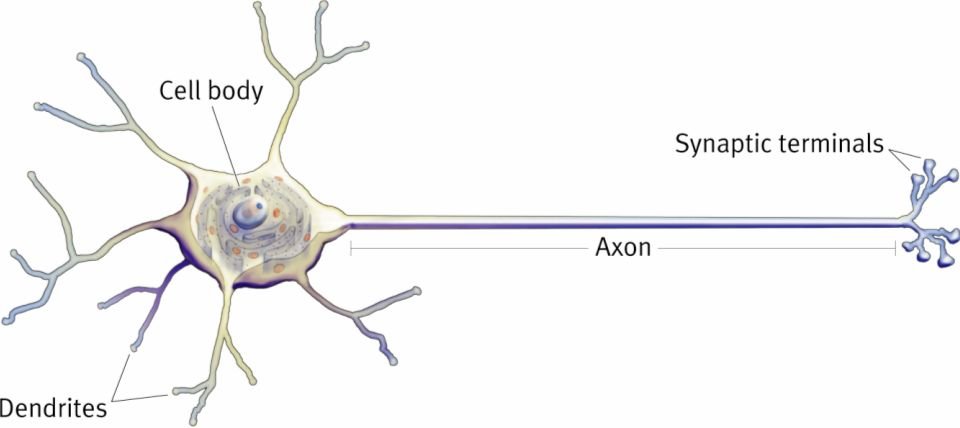
\includegraphics[width=0.8\textwidth,scale=1]{files/neuron.jpg}  
\caption{The parts of a nerve cell or neuron as shown in \cite{NEU}.}
\label{fig:neuron}
\end{figure}
\end{center}


\section{Mathematical formalisation}\label{sec:mcpitts}
During the second world war, research in computer technology has been promoted for the sake of military purposes. With the advent of computer technology, neural networks started to become significant as models of abstract automata. McCulloch and Pitt's 1943 published work (>>\textit{A logical calculus of the ideas immamnent in nervous activity}<<) proposes a cell which allows th simulation of AND-, OR- and NOT-gates and therefore every boolean function. This cell is a simple model of neuron with binary threshold and the first formal describtion of a neural network. Within their work, neurons are perceived as basic Input/Ouput units, which process input of $i$ neurons and propagate their output further into the network through a single output.\\

The activity level $a_j$ of a neuron $j$ is assigned by its transfer function $\varphi$. McCulloch and Pitt proposed a simple step function, where $S$ is the threshold:\\

\begin{equation}
	\varphi(x)=\begin{cases}
		0: \quad  x < S \\
		1: \quad  x \geq S \\
	\end{cases}
\label{eq:step}
\end{equation}
%The synaptic terminal's function is depicted by the multiplication of the input from neuron $a_i$ by a factor, the weight $w_{ij}$ of the connection link between neurons $i$ and $j$. $w_{ij}$ is either excitatory or inhibitory. 
Given the definition of $\varphi$ in equation \eqref{eq:step}, activity levels are always binary and computed as follows:\\

%\begin{equation}
%a_j = \varphi(\sum_{i=0}^{} w_{ij} \cdot a_{i}), \quad a_i \in \{0, 1\}, w_{ij} \in \{1, -1\}
%\end{equation}

\begin{equation}
a_j = \varphi(\sum_{i}^{} a_{i}), \quad a_i \in \{0, 1\}
\end{equation}

Figure \ref{fig:mathneuron} illustrates the mathematical formalisation proposed in \cite{MATHNEURON}. This model has later been named \textbf{McCulloch-Pitts neuron}. 


\begin{figure}[H]
\centering

\begin{tikzpicture}
\node [align=center] (in1) at (-0.5,0) {$a_i$}; 
\node [align=center] (in2) at (-0.3,0.75)   {}; 
\node [align=center] (in3) at (-0.8,1.5) {$a_i = 1$}; 
%\node [align=center] (w1) at (0.7,0) {$w_{ij}$}; 
%\node [align=center] (w3) at (0.7,1.5) {$w_{0j}$};
\node [align=center] (input) at (2,0.75) {\ \ $\sum_{}^{in_{j}}$}; 
\node [align=center] (function) at (4,0.75) {$\varphi$}; 
\node [align=center] (output) at (6,0.75) {$a_j$}; 
%\node [align=center] (o1) at (8.5,0) {};
\node [align=center] (o2) at (8.5,0.75) {};
%\node [align=center] (o3) at (8.5,1.5) {};

\node [align=center] (desilinks) at (-0.60,-1) {Input\\ Links}; 
\node [align=center] (desinput) at (1.9,-1) {Input\\ funcion}; 
\node [align=center] (desfunc) at (4,-1) {Activation\\ function}; 
\node [align=center] (desoutput) at (6,-1) {Output}; 
\node [align=center] (desolinks) at (8,-1) {Output\\ link}; 

\node [align=center] (desweight) at (4,2) {$a_j = \varphi(in_j)$}; 
%\node [align=center] (desinfunc) at (0.75,2) {\small Weight}; 
\node [align=center] (descneuron) at (6,1.5) {\small Cell body}; 

\node [align=center] (dummy1) at (2.4,0.75) {}; 
\node [align=center] (dummy2) at (5.36,0.75) {}; 

\draw[arrow]	(in1) -- (input);
\draw[arrow]	(in2) -- (input);
\draw[arrow]	(in3) -- (input);

%\draw[arrow]	(output) -- (o1);
\draw[arrow]	(output) -- (o2);
%\draw[arrow]	(output) -- (o3);

\node[draw=black,fit=(dummy1) (function) (dummy2) ,ellipse] (tmp) {};

\end{tikzpicture}
\caption{A mathematical model of a neuron $j$}
\label{fig:mathneuron}
\end{figure}

This proposal is of particular importance for the theory of ANN and inspired significant researchers like John von Neumann or Nobert Wiener, who developed cybernetics. However, the McCulloch-Pitts neurons are limited by their inability to learn, resulting from their fixed structure. They also lack the surprising robustness of biological nerve networks, since they rely on a flawless operation of all components. Nevertheless, they still have significance in electrical engineering, where they are used to realise binary functions, due to their increased efficiency in contrast to gates. 

\chapter{Artificial neural networks}
\section{Overview}

Scientists have proposed a multitude of different network structures since the advent of reasearch in ANN through their first formalisation. A lot of which have been designed with various motivations, stemming from the differnent perception of neural networks across disciblines. Categorisation can be achieved by distinguishing several parameters, e.g. the number of layers, acceptance of input types or usage of learning techniques. Figure \ref{fig:class} illustrates a possible categorisation\cite{NNGER}. The direction of signal flow serves as a first level of distinction, as it substantially characterises the networks structure, complexity and so on. Both types of signal flow mandate the propagation of network input further into the network. Feedforward network prohibit the usage of non-straightforward signal flow, i.e. connections may only emerge between subsequent neurons. Any connections to predecessors are forbidden. This constraint has allowed for a quick development of learning techniques, empowering ANN to learn from data. 

As distinct from feed-forward networs, recurrent (or feedback) networks allow bidirectional signal flow. As links from one neuron may be formed with any other neuron in the network, recurrent network are often categorised by increased complexity. As the current state of a neuron may be continously changing, recurrent networks demand advanced learning algorithms. Due to their dynamic nature, they allow for the modelling of advanced techniques, such as long and short term memory.

\begin{figure}[H]
\centering

\fbox{
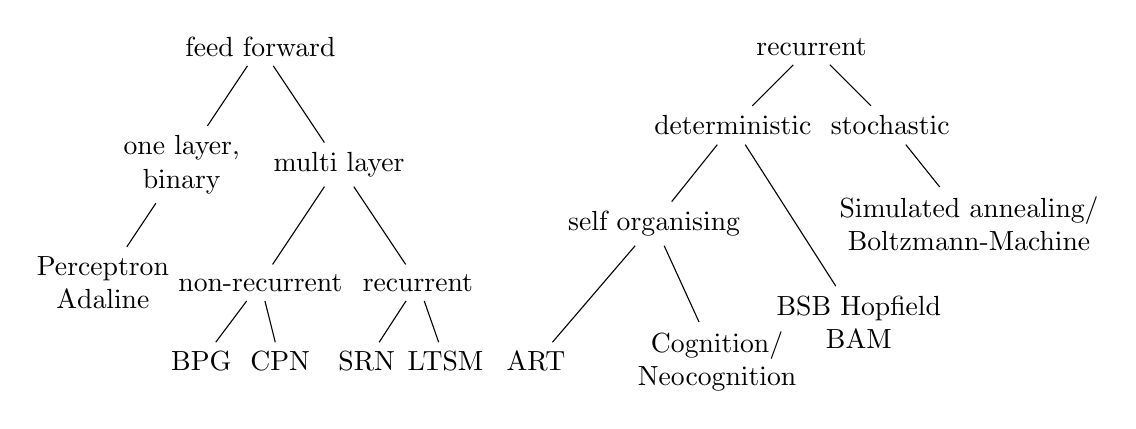
\begin{tikzpicture}
\node [align=center] (L1) at (3,10) {feed forward}; 

\node [align=center] (R1) at (10,10) {recurrent}; 


\node [align=center] (L21) at (2,8.5) {one layer,\\ binary}; 
\node [align=center] (L22) at (4,8.5) {multi layer}; 

\node [align=center] (R21) at (9,9) {deterministic}; 
\node [align=center] (R22) at (11,9) {stochastic}; 


\node [align=center] (L31) at (1,7) {Perceptron\\Adaline}; 
\node [align=center] (L32) at (3,7) {non-recurrent}; 
\node [align=center] (L33) at (5,7) {recurrent}; 

\node [align=center] (R31) at (8,7.75) {self organising}; 
\node [align=center] (R32) at (10.6,6.5) {BSB Hopfield\\BAM}; 
\node [align=center] (R33) at (12,7.75) {Simulated annealing/\\Boltzmann-Machine}; 


\node [align=center] (L41) at (2.25,6) {BPG}; 
\node [align=center] (L42) at (3.25,6) {CPN}; \node [align=center] (L43) at (4.35,6) {SRN}; 
\node [align=center] (L44) at (5.35,6) {LTSM}; 

\node [align=center] (R41) at (6.5,6) {ART}; 
\node [align=center] (R42) at (8.80,6) {Cognition/\\Neocognition}; 

\foreach \s/\t in {L1/L21,
                   L1/L22,
                   L21/L31,
                   L22/L32,
                   L22/L33,
                   L32/L41,
                   L32/L42,
                   L33/L43,
                   L33/L44}
    \draw (\s) -- (\t);

\foreach \s/\t in {R1/R21,
                   R1/R22,
                   R21/R31,
                   R21/R32,
                   R22/R33,
                   R31/R41,
                   R31/R42}
    \draw (\s) -- (\t);

\end{tikzpicture}}
\caption{A categorisation of neural network types. BPG = Bachpropagation, CPN = Counterpropagation, BAM = Bidirectional associative memory, BSB = Brain-State-in-a-Box, ART = Adaptive Resonance Theory, SRN = Simple recurrent network, LTSM = Long short term memory}

\label{fig:class}
\end{figure}
A comprehensive introduction of all categorised network types would exceed the scope of this project work, and therefore only a subset, interesting for the particular application, will be introduced. Within this chapter, I will give an introduction of the terminology and mathematical models used to represent a neural network on a computing machine. An appraisal of advantages and detriments of the presented models is rather difficult, as their performance hugly depends on the specific application. Regarding machine learning, and thereforea also ANN, the term performancedemands for a new definition. Machine learning is a scientific discipline that explores the construction and study of algorithms that can learn from data.\cite{MLDEF1} Such algorithms operate by building a model from example inputs and using that to make predictions or decisions.\cite{MLDEF2} As distict from other algorithms, there can never be absolute certainity of the correctness of a machine learning model. This stems from their usage of the probability of statistics applied to real world problems. Algorithmic measures, such as optimality and completeness cannot be utilised to assess the usefulness of a machine learning technique. A performance evaluation can therefore only be conducted given a specific problem and the according data. After all, the selection and appropriate usage of neural network structures requires extensive experience and/or thorough testing. 

\section{Network structure}
\subsection{Layers}
The units within a network are categorised into several layers according to their position. This allows for an accurate describtion of the network and the function of each respective unit within the network. The set of layers of a ANN will be denoted as $L$, where an artificial neural network of size n, written as $\text{ANN}^n$ is the union of the n layers in the network:

\begin{equation}
    \text{ANN}^n = \bigcup_{N}^{i=1}{L_i}
\end{equation}

The amount of neurons within a layer is equal to the elements of the respective set. The total number of neurons in an ANN is $\sum_{i=1}^{n}{|L_i|}$. The tuple $(|L_1|,...,|L_n|)$ is called the \textbf{network topolgy} and fully describes the stucture (with exclution of the connections) of a feed-forward network. Recurrent networks need and additional describtion.

The first network layer $L_1$, is referred to as the the input layer. It receives the input vector $\overrightarrow{x} \in \mathds{R}^{|L_1|}$ and passes it onto the next layer. Likewise, $L_n$ is the output layer of the network, whose neurons are called the output units. $\overrightarrow{y} \in \mathds{R}^{|L_n|}$ is the output vector of an ANN. A computer application will later utilise the neural network as a black box, being only interested in the transformation from $\overrightarrow{x}$ to $\overrightarrow{y}$. Figure \ref{fig:layer} shows this. 

\begin{figure}[H]
\centering

\begin{tikzpicture}
\node [draw=black, align=center, circle] (i1) at (0,3) {}; 
\node [draw=black, align=center, circle] (i2) at (0,2) {}; 
\node [draw=black, align=center, circle] (i3) at (0,1) {}; 
\node [draw=black, align=center, circle] (i4) at (0,0) {}; 

\node [draw=black, align=center, circle] (h01) at (2,2.5) {}; 
\node [draw=black, align=center, circle] (h02) at (2,1.5) {};
\node [draw=black, align=center, circle] (h03) at (2,0.5) {};

\node [draw=black, align=center, circle] (h1) at (4,2.5) {}; 
\node [draw=black, align=center, circle] (h2) at (4,1.5) {};
\node [draw=black, align=center, circle] (h3) at (4,0.5) {};

\node [draw=black, align=center, circle] (o1) at (6,2) {};
\node [draw=black, align=center, circle] (o2) at (6,1) {};

\draw[arrow]	(i1) -- (h01);
\draw[arrow]	(i1) -- (h02);
\draw[arrow]	(i1) -- (h03);

\draw[arrow]	(i2) -- (h01);
\draw[arrow]	(i2) -- (h02);
\draw[arrow]	(i2) -- (h03);

\draw[arrow]	(i3) -- (h01);
\draw[arrow]	(i3) -- (h02);
\draw[arrow]	(i3) -- (h03);

\draw[arrow]	(i4) -- (h01);
\draw[arrow]	(i4) -- (h02);
\draw[arrow]	(i4) -- (h03);

\draw[arrow]	(h1) -- (o1);
\draw[arrow]	(h1) -- (o2);

\draw[arrow]	(h2) -- (o1);
\draw[arrow]	(h2) -- (o2);

\draw[arrow]	(h3) -- (o1);
\draw[arrow]	(h3) -- (o2);

\node[draw=black,fit=(i1) (i2) (i3) (i4),ellipse] (inputLayer) {};
\node[draw=black,fit=(h01) (h02) (h03) ,ellipse] (hiddenLayer) {};
\node[draw=black,fit=(h1) (h2) (h3) ,ellipse] (hiddenLayer) {};
\node[draw=black,fit=(o1) (o2) ,ellipse] (outputLayer) {};

\node [align=center] (x) at (-1,1.5) {$\overrightarrow{x}$};

\node [align=center] (di) at (0,5) {\textcolor{black}Input\\ layer\\ $L_1$};
\node [align=center] (dh1) at (2,5) {\textcolor{black}Hidden\\ layer\\ $L_{2}$};
\node [align=center] (dh1) at (3,1.5) {$\cdots$};
\node [align=center] (dh2) at (4,5) {\textcolor{black}Hidden\\ layer\\ $L_{n-1}$};
\node [align=center] (do) at (6,5) {\textcolor{black}Output\\ layer\\ $L_n$};

\node [align=center] (y1) at (7,1.5) {$\overrightarrow{y}$};

\end{tikzpicture}
%\caption{%An example of an artificial neural network with $n$ layers. Its network topology is $(|L_1|=4,|L_2|=3,...,|L_{n-1}|=3,|L_n|=2)$}
\label{fig:layer}
\end{figure}

Praticular significance is drawn to the layers in between input and output layer. Those layers are optional, but needed to solve certain problems. We will discuss the importance of hidden layers for problem solution in chapter \ref{chap:nets}. We denote the set of hidden layers as $H$. It is described as follows:
\begin{equation}
H \subseteq L; H = \{L_i|1<i<n\}
\end{equation}

\subsection{Units}

A first improvement to McCulloch and Pitt's model was the concept of weights on the connecting links. Inspired by the function of the synaptic terminals, a weight $w_{ij}$ between two neurons $n_i$ and $n_j$, models the magnitude of influence. Weights may be both positive and negative, exhibatory or inhibatory. A magnitude of zero stands for a cut-off signal flow. The entirety of connection weights wihin a network is often sored in a matrix, which allows for performant manipulation. The manipulation of connections weight may be used to alter the network's behaviour. $W$ is called the connection matrix, which fully represnts the structure of a feed-forward network with $i$ layers:
\begin{equation}
W = 
\begin{pmatrix}
w_{11} & \cdots & w_{i1} \\
\vdots & \ddots & \vdots \\
w_{1j} & \cdots & w_{ij} \\
\end{pmatrix}
\end{equation}

In addition, the concept of bias neurons has proven itself useful. Bias units are non-receptive, both in feed-forward and recurrent networks. Hence their activity level is steady, usually $+1$. Links between bias and normal neurons are to be treated normally, the influence of a bias can therefore be altered. They are often used to keep units with little weighted input active, by shifting their activation function $\varphi$ they don't receive significant input. In contrast, a negative link may be used to keep a neuron in an inactive state.
\begin{figure}[H]
\centering

\begin{tikzpicture}
\node [draw=black, align=center, circle] (i) at (0,0) {$n_0$}; 

\node [draw=black, align=center, circle] (o) at (4,0) {$n_1$}; 

\draw[arrow]	(i) -- (o);

\node[] (dw) at (2,0.3){$w_{ij}$};
\node[] (di) at (0,0.6){Input: $x$};
\node[] (do) at (4,0.6){Output};
\node[] (df) at (2.1,-0.7){$\varphi = sig(w_{01}\cdot x)$};
\end{tikzpicture}
\caption{A single input-output network}
\label{fig:1on1}
\end{figure}

Consider the network shown in figure \ref{fig:1on1}. The activation function of the output neuron is chosen to be the sigmoid function. Figure \ref{fig:sigmoid-scale} shows the output for several values of $w$. It can seen that $w$ changes the steepness of the sigmoid function. 

\begin{figure}[H]
    \centering
    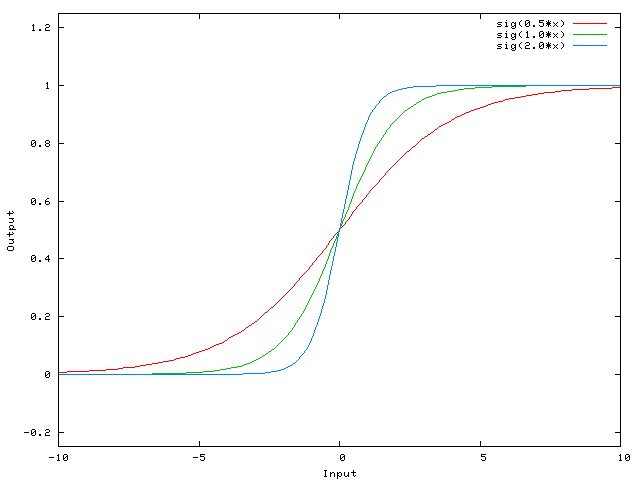
\includegraphics[width=0.65\textwidth,scale=1]{files/sigmoid-scale.png}  
    \caption{The output of unit $n_1$ in figure \ref{fig:1on1}}
    \label{fig:sigmoid-scale}
\end{figure}


Figure \ref{fig:2on1} shows the same network with an additional bias neuron. This allows us to shift the activation function according to the weight of the connection link $w_{12}$ as shown in figure \ref{fig:sigmoid-shift}.

\begin{figure}[H]
\centering
\begin{tikzpicture}
\node [draw=black, align=center, circle] (i2) at (0,2) {$n_0$}; 
\node [draw=black, align=center, circle] (i1) at (0,0) {$n_1$}; 
\node [draw=black, align=center, circle] (o) at (4,1)  {$n_2$}; 

\draw[arrow]	(i2) -- (o);
\draw[arrow]	(i1) -- (o);

\node[] (dw) at (2,1.8){$w_{02}$};
\node[] (dw) at (2,0.8){$w_{12}$};
\node[] (di) at (0,0.6){Bias: $1.0$};
\node[] (di) at (0,2.6){Input: $x$};
\node[] (do) at (4,1.6){Output};
\node[] (df) at (2.1,-0.7){$\varphi = sig(w_{02}\cdot x + w_{12}\cdot 1.0)$};
\end{tikzpicture}
\caption{A single input-output network}
\label{fig:2on1}
\end{figure}

\begin{figure}[H]
    \centering
    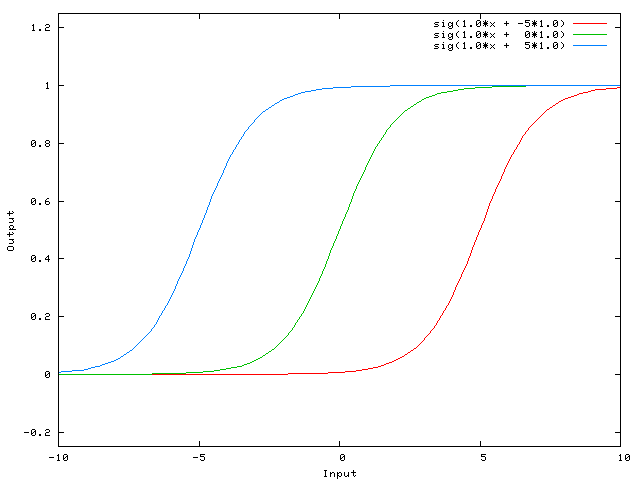
\includegraphics[width=0.65\textwidth,scale=1]{files/sigmoid-shift.png}  
    \caption{The output of unit $n_1$ in figure \ref{fig:2on1}}
    \label{fig:sigmoid-shift}
\end{figure}

\subsection{Activation functions}

As discussed before, the weights of the connections between the neurons represent the 'Intelligence' of the network. The bigger the absolute value of the weight, the greater the influence of a neuron to another. This value can be both positive and negative, as well as neutral \textit{(0)}, meaning that there is currently no influence between the neurons, although there is still a link connecting them. A weight of 0 can be understood as a logical pinch of the link, preventing it from transmitting signals.




The connection between the input values and the activity level of the neuron is made by the activity function $\varphi$. Different models are obtained depending on the choice of the activity or transfer function. Amongst the most common choices are the linear, binary step and sigmoid function as illustrated in Figure \ref{fig:plots}. The linear function has a threshold $t$, which can be used to avoid low network input (e.g. noise) to be further propagated into the network. The binary step function represents the firing of a pulse down the axon if positive $1$), while $0$ represents no firing. The step function is sometimes defined to jump from $-1$ to $1$. 

Sigmoid functions are widely used amongst network which are to represent cognitive processes such as perception, recognition, problem solving, etc. .
Both the logistic function as well as the hyperbolic tangent function $\tanh()$ can be used. The main advantage of sigmoid functions are:

\begin{itemize}
\item In contrast with the linear function (without a threshold), the activity level of the function is limited in both the positive and the negative. This means that activity in the network can not spill over unintentionally, which can be caused by recurrent connections.
\item Differentiability
As distinct from the binary step function, it is differntiable at all parts, which as an example, is a requirement of the gradient descent, used by the backpropagation algorithm (about to be introduced in section \ref{sec:learning}
\end{itemize}


\begin{figure}[H]
\centering
\subfigure[]
{
   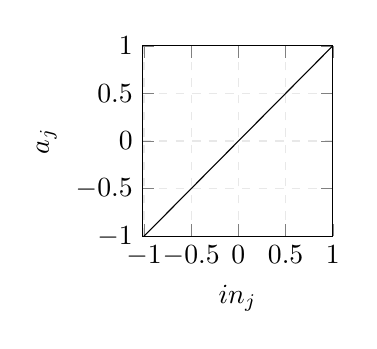
\begin{tikzpicture}
		\begin{axis}[
        width=4cm, height=4cm,
        grid = major,
        grid style={dashed, grey!30},
		xmax=1,        
        ymin=-1,
        ymax=1,
        axis background/.style={fill=white},
        ylabel=$a_{j}$,
        xlabel=$in_{j}$]
     
		\addplot[black]{x};
		\end{axis}
	\end{tikzpicture}
\label{fig:plot1}
}

\subfigure[]
{
   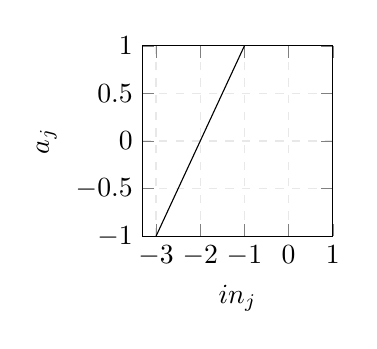
\begin{tikzpicture}
		\begin{axis}[
        width=4cm, height=4cm,
        grid = major,
        grid style={dashed, grey!30},
		xmax=1,        
        ymin=-1,
        ymax=1,
        axis background/.style={fill=white},
        ylabel=$a_{j}$,
        xlabel=$in_{j}$]
     
		\addplot[black]{x+2};
		\end{axis}
	\end{tikzpicture}
\label{fig:plot2}
}

\subfigure[]
{
   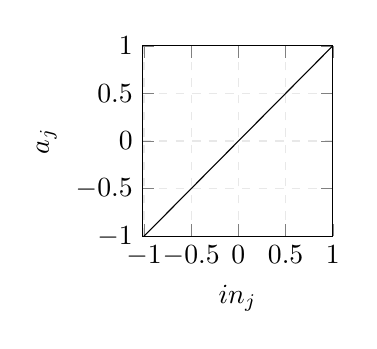
\begin{tikzpicture}
		\begin{axis}[
        width=4cm, height=4cm,
        grid = major,
        grid style={dashed, grey!30},
		xmax=1,        
        ymin=-1,
        ymax=1,
        axis background/.style={fill=white},
        ylabel=$a_{j}$,
        xlabel=$in_{j}$]
     
		\addplot[black]{x};
		\end{axis}
	\end{tikzpicture}
\label{fig:plot2}
}
	
\caption{Comparison of commonly used activation functions}
\label{fig:plots}
\end{figure}

In order to teach neural networks and enable them to apply learned behavior in following scenarios, the work with them is divided in a training- and test phase. During the training, the network learns certain behavior by feeding repetitive input to the first layer and observing the output of the network. This can be done in a supervised and unsupervised way. In a supervised training phase, the targeted output of the network is already known and is presented to the network as a \textit{teaching factor}. The network produces output depending on the current weights on its connections and adjusts them according to the margin between the targeted and produced output. Unsupervised learning is necessary in situations, where no reasonable teaching factors are available or the observant is more interested on the performance. Similarity between input incentives and connection weights is the factor, according to which weight adjustment is done in such models.

\section{Applications}
Until today, neural networks have been successfully applied to several problems in a variety of scientific and industrial applications. Although of greatly different nature, almost all of those applications can be reduced to either pattern/shape recognition or logical filter tasks. Examples are:\\
\begin{itemize}
    \item On-line recognition of handwritten text
    \item Autopilots in aerospace engineering
    \item Noise suppression and signal filtering in communication technology 
    \item Object recognition
    \item Weather forecast
    \item Function approximation including time series prediction
\end{itemize}

The following sections will give a brief notion of some 'classical' applications where ANNs have found better solutions in quicker time in comparison with other techniques.
\subsection{Recognition of hand-writing}
The automated interpretation of hand-written is of great interest for a number of purposes. The destination address of letters and parcels are nowadays processed by computers which use real-time images to recognise letters. The typesetting system \LaTeX allows its users to write complex formulas using certain commands that are later being replaced by symbols such as the existential quantifier $\exists$. One would now wish for a system that can take in a hand written representation of the symbol and output the command by which the symbol can later be written in a document. In \cite{MARTIN} artificial neural networks are used to classify such symbols. The user is then presented a choice of matching symbols and their commands associated with a probability measure of their correctness. The website is available under \url{write-math.com}.
\\

The challenge for such systems is the great deviation between different styles of hand writing. This makes it virtually infeasible for other conventional methods to reliably classify hand-writing. The network model RCE - Restricted Coulomb Energy Network has been devised by Nobel price winner Leon Cooper. It overcomes the limitations of the Perceptron as it is capable of detecting geometrical figures (therefore also handwritten text) of any size. Cooper's company Nestor, has successfully used this model to develop a system which can detect characters of the Japanese alphabet Kanji. The Kanji alphabet stems from the Chinese language, contains approximately 3000 different symbols and is extremly complex. Examples are \begin{CJK}{UTF8}{min}輸\end{CJK} - transport or \begin{CJK}{UTF8}{min}熊\end{CJK} - bear. It is nowadays extensively used on mobile devises that allow to write text messages by drawing each individual character instead of choosing symbols from a massive dictionary. Complex sentences formulated by simultaneously using three different alphabets, such as \begin{CJK}{UTF8}{min}世界はコンピュータ技術の登場以来、劇的に変化した。\end{CJK} - \textit{The world has changed dramatically since the advent of computer technology} can now be written in a fairly short amount of time.

\subsection{The Travelling-Salesman-Problem}
Given a set of cities and the distances between each pair of cities, what is the shortest path that, after visiting each city exactly once, leads to the origin of the route? This task, called the Travelling-Salesman-Problem (short: TSP) is an optimisation task which is often encountered in practice (Energy and water supply, microchip design). The TSP can be modelled as a graph: All $n$ cities are represented as vertices, the connections between the cities as edges. Since all cities are connected with each other, the graph is complete. A complete graph is called $K_n$. The cost (travel time) between each pair of vertices $i$ and $j$ is associated with a weight $w(i,j) \geq 0$. A tour that visits each city once and return back to the origin is a Hamilton-circle. As the graph is complete, there are several Hamilton-circles (each of which is a possible solution of the problem). Each permutation of the nodes is a Hamilton-circle, thus there are $n!$ circles. Sought is the Hamilton-circle with the least overall cost, i.e. a permutation $\pi(1),\dots,\pi(n)$ with minimal weight
\begin{equation}
    \sum\limits_{i=1}^n w(\pi(i),\pi(i+1)), 
\end{equation}

where $\pi(n+1)$ is set to $\pi(1)$.\cite{MATHINF}\\

It is of high importance to theoretical computer science, as it is known to be $NP$-complete. In the field of complexity analysis, the class of decision problems for which there is a deterministic Turing-Machine able to solve it in time $\mathcal{O}(n^k)$ is called $P$ (polynomial). An example is the sorting problem. Class $P$ contains problems with running times like $\mathcal{O}(n)$ and $\mathcal{O}(log(n))$ but also those with time $\mathcal{O}(n^{5000})$. In addition to the deterministic Turing machine, complexity analysis also defines the non-deterministic Turing machine. At each time step, there are several possible ways of continuing computation, setting it in contrast with todays computers. The class of Problems $NP$ is solvable by a non-deterministic Turing Machine in polynomial time. $NP$ contains a number of relevant problems, such as the graph isomorphism (Can two graphs be drawn identically?). Problems in $P$ can also be solved by this theoretical model, so $P \subseteq NP$. In other words, a problem is in the class of NP if there is an algorithm (executed by a Turing machine) that can guess a solution and verify whether the guess was correct in polynomial time. In case of omniscient guessing or given a number of processors equal to the number of solutions, trying out all possibilities at the same time one would always get the correct solution. Thus, $NP$ problems would become $P$ problems. 

Nevertheless, computationally feasible approximation techniques have been found which allow to find a good, although not always the best, solution. Hopfield and Tank (1985) proposed an approach using ANNs which allows to find a good, often even the best solution for the TSP. It suggests a single-layer network with $n$ neurons, where $n$ equals the number of cities in the graph, called Hopfield-network. This can be thought of as a square with an edge length of $n$The output of each individual neuron equals the time step at which the city is visited. 







\chapter{Learning}\label{sec:learning}
\section{Hebbian learning rule}
The psychologist Donald Olding Hebb proposed on the easiest learning rules with high biological plausibility in \cite{HEBB}:\\

\textit{“Let us assume that the persistence or repetition of a reverberatory activity (or "trace") tends to induce lasting cellular changes that add to its stability.… When an axon of cell A is near enough to excite a cell B and repeatedly or persistently takes part in firing it, some growth process or metabolic change takes place in one or both cells such that A's efficiency, as one of the cells firing B, is increased.”}\\

In summary: The weight between two units $i$ and $j$ is changed, if both units are active at the same time. The amount of change is set by three factors:

\begin{itemize}
\item The activity level of the sending unit $a_i$.
\item The activity level of the receiving unit $a_j$.
\item A settled and constant parameter $\eta$
\end{itemize}

The weight change $\Delta w_{ij}$ using the bias learning rule is shown in equation \eqref{eq:hebb}.
\begin{equation}
\Delta w_{ij} = \eta \cdot a_i \cdot a_j
\label{eq:hebb}
\end{equation}

One of the major drawbacks of the Hebbian rule is the fact, that is can only applied on networks without a hidden ayer, and therefore only very simple neural networks.

\section{Delta rule}
The delta rule is based on the comparison between a targeted output $t$ and the observed output $o$ and can therefore only be applied with supervised learning.
It can be expressed using equation \eqref{eq:delta1}.
\begin{equation}
\delta = t - o
\label{eq:delta1}
\end{equation}

The following possibilities can be observed:
\begin{itemize}
\item \textbf{The observed output is too low}\\
In order to amplify the output, the weights between neurons is strengthened, provided a positive weight on the connection linking them. Negative weights are weakened.
\item \textbf{The observed output is too high}\\
All connections with positive weights are weakened, while the ones with negative weights are strengthened 
\item \textbf{Targeted and observed output are equivalent. (= ideal behavior)}\\ There is no need to change the links.
\end{itemize}

The deltas learning rule equation \eqref{eq:delta2} covers all three possibilities, thus ensuring that the changing rate is proportional to the difference between targeted and observed. The learning parameter $\eta$ is again set before the beginning of the learning process and remains constant. The multiplication with the sending units output $a_i$ ensures that those connections, that have the greatest influence into the error have the greatest $\delta w_{ij}$.
\begin{equation}
\Delta w_{ij} = \eta \cdot \delta \cdot a_i
\label{eq:delta2}
\end{equation}

The simplicity of this learning rules also comes at great cost: The comparison only allows us to adjust connections which connect to the rightmost layer in the network. This fact restricts the application of this method from networks with a hidden layer. 

\section{Backpropargation}

\subsection{Gradient descent}

The optimisation algorithm gradient descent (also steepest descent) tackles the problem of finding a local minimum of a multivariable function $F(x)$. In order to do, one substracts the gradient $\nabla F(a)$ from the current point $a$ to obtain a new point $b$ so that $F(a) \geq F(b)$. The non-negative weight $\gamma$ is often referred to as the stepsize.

\begin{equation}
 b = a - \gamma \nabla F(a)
\label{eq:graddes}
\end{equation} 

The gradient of a differentiable function $f: D \subseteq \mathds{R}^n$ $\rightarrow$ $\mathds{R}$ must disappear at a local minimum or maximum at $x_i$:\cite{MATHINF}

\begin{equation}
\nabla F(x_i) = 0
\end{equation} 

Starting with guess $x_0$ for a local minimum, and iteratively calculating an $x_{i+1}$ according to equation \eqref{eq:graddes}, we will obtain $x_0, ..., x_i$ so that $F(x_0) \geq F(x_1) \geq ... \geq F(x_{n-1}) \geq F(x_n)$. The parameters $\theta$ and $n$ are  used as an ending criteria for the algorithm. Algorithm \ref{alg:GD} shows the complete algorithm.

\begin{algorithm}[H]
\LinesNumbered
\DontPrintSemicolon
\BlankLine
\Ein{A differentiable function $F(x)$, stepsize $\gamma$, tolerance $\theta$, point $x_0$}
\Aus{A local minimum at $x_i$}
\BlankLine
\Begin
{
    \Repeat{$\Delta x < \theta$ for $n$ iterations}
    {
        $x_{i+1}$ = $x_i - \gamma \nabla F(x_i)$
    }
}
\caption{The gradient descent algorithm}
\label{alg:GD}
\end{algorithm}

Gradient descent may be imagined as the effort of a wanderer to reach the bottom of valley as quick as possible, therefore always seeking to climb down as the point of steepest descent. This is illustrated in Figure \ref{fig:grad}

\begin{figure}[H]
    \centering
    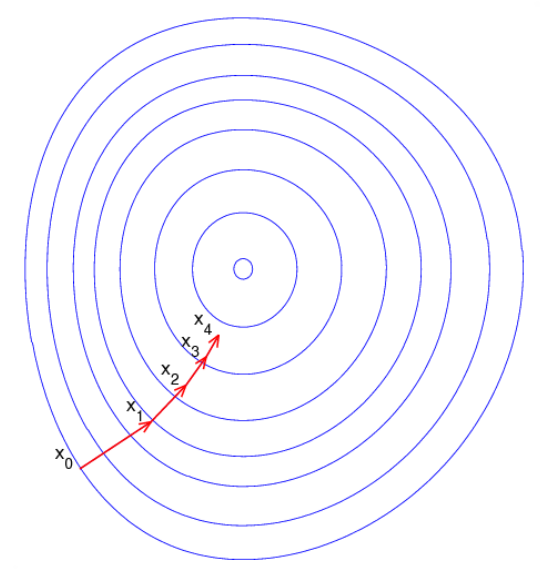
\includegraphics[width=0.3\textwidth,scale=1]{files/graddes.png}  
    \caption{Illustration of gradient descent.\cite{GRADFIG}}
    \label{fig:grad}
\end{figure}

\subsection{The backpropagation algorithm}

The backpropargation algorithm is yet another learning rule for supervised networks, but in comparison to the hebbian and delta rules, it can also be applied for networks with $n$ numbers of hidden layers. There are certain problems that cannot be solved by networks without at least one hidden layer, the XOR-Gate being an famous example for such problems. It was first devised by Paul Werbos in 1975 \cite{BACK} and consists of three stages:
\begin{itemize}
\item[1.] \textbf{The forward-pass}:
A pattern is presented to the input layer and further propargated into the network.
\item[2.] \textbf{Error-determination}:\\
The observed output is compared to targeted result and an error $E$ is determined by a derivale error-function $\varphi$ shown in equation \eqref{eq:backerror}. The factor of $\frac{1}{2}$ is used to simplify the derivation by cancelling the exponent.

\begin{equation}
\varphi = \frac{1}{2} (t-o)^2
\label{eq:backerror}
\end{equation}
\item[3.] \textbf{Backward-pass}:\\
The error is propargated from the back of the network to the front, hence the name \textbf{Backpropargation}. The connection are updated independent from their influence to $E$, which guarantees a result $o$ that is closer to $t$, provided the same output is presented to the input layer.
\end{itemize}

A first approach on finding a method to changing all weights in a weight that will minimize the error is to find $E$ for all possible combinations of weights $W$. The combination $W_{min}$ with the smallest $E$ would be the perfect solution, an abolute minimum of the error. The problem of this approach is that the computitional effort to finding this solution is way to high, since $W_{min}$ would have to be found in a $n$-dimensonial  hyperplane (given the number of neurons $n$).\\

Instead, the weights are adjusted using the gradient descent, which does not need to know the complete hyperplane\marginpar{\textit{gradient descent}}. It starts with a random combination of weights for which the gradient is determinded. The gradient is the function of a scalar field which shows the rate of change and the direction of the greatest change in the form of a vector field. After the gradient is determined it will be stepped down at a given rate - the learning rate, meaning that the weights are adjusted. For this new combination of weights, the gradient is again determined and stepped down until a local (or global minimum) is found or a maximum amount of repetitions is reached.\\

The amount of change between neurons $i$ and $j$ $\delta w_{ij}$ is calculated as shown in \eqref{eq:backrule}.
\begin{equation}
\Delta w_{ij} = -\eta \frac{\partial E}{\partial w_{ij}} = \eta \cdot \delta_j \cdot a_i
\label{eq:backrule}
\end{equation}
As distinct form the delta rule, the backpropargation rule differs two cases, shown in equation \eqref{eq:backcases}. $k$ is the index of the neurons in the subsequent layer.
\begin{equation}
   \delta_j =
   \begin{cases}
     \varphi'(in_j)(t_j-o_j) & \text{In case j is an output neuron} \\
     \varphi'(in_j)\sum_{k} \delta_k \cdot w_{j,k} & \text{In case j is a hidden neuron}
   \end{cases}
\label{eq:backcases}
\end{equation}

Eventually, the weights are changed acording to equation \eqref{eq:backweight}.

\begin{equation}
   w_{ij}^{new} = w_{ij}^{old} + \Delta w_{ij}
\label{eq:backweight}
\end{equation}

\section{Backpropargation through time}
\section{Competitive learning}
%...
\chapter{Network types}\label{chap:nets}
At the moment there are three generations of neural networks. 
The first generation works with binary in- and outputs, but real thresholds. The first model was presented in 1943.
In the second generation, presented in the 90s, the firerates symbolizes real values transmitted on in- and outputs. Real thresholds are still used.
The newest generation uses spikes, an encoding through time.

\subsection{First generation}
The first generation of neural networks have binary in- and outputs.

\subsubsection{McCulloch-Pitts neuron}
The first mathematical model of a neuron was the McCulloch-Pitts-neuron,
developed by Warren McCulloch and Walter Pitts in 1943.
They wanted to realise a simple, realistic neuron-modell of operations in the brain and find out if the brain could compute turing computability functions.
McCulloch-Pitts-neuron has binary in- and outputs.
A real threshold can be defined, which reached, let the neuron fire an one, otherwise zero.
Its possible to add absolute suppressing inputs. If one of these has the value one, the neuron gives out zero, no matter of other inputs. The use of such absolute supressing inputs is for the most cases doubtfull.


Neural networks of this type of neuron can just learn by changing topology of the network, that is laborious.

At the following a figure of a single neuron:

\begin{figure}[H]  % [H] erzwingt Position an der Stelle im Text
	\centering
	\begin{tikzpicture}
	\node [align=center] (dummy1) at (-0.25,3.5) {$x_{1}$}; 
	\node [align=center] (dummy2) at (-0.25,2.5) {$x_{n}$}; 
	\node [draw=black, fill=white, align=center, circle] (f1) at (1,3) {f}; 		
	\node [align=center] (dummy3) at (3,3) {f($x_{1}$,..,$x_{n}$)}; 
	\draw[arrow]	(dummy1) -- (f1);
	\draw[arrow]	(dummy2) -- (f1);
	\draw[arrow]	(f1) -- (dummy3);
	\draw[dotted] (dummy1) -- (dummy2);
	
	\end{tikzpicture}
	\caption{A McCulloch-Pitts-neuron}
	\label{fig:pitts1}
\end{figure}
The neuroninput is computed by:

\begin{equation}
	neuroninput = \sum_{i=1}^{n} x_{n} \quad  x \in \{0, 1\}
\end{equation}


A function composition:

\begin{figure}[H]
	\centering
	\begin{tikzpicture}
	\node [align=center] (dummy1) at (-0.25,3.5) {$x_{1}$}; 
	\node [align=center] (dummy2) at (-0.25,2.5) {$x_{n}$}; 
	\node [draw=black, fill=white, align=center, circle] (f1) at (1,3) {f}; 		
	\node [draw=black, fill=white, align=center, circle] (g1) at (2.5,3) {g}; 
	\node [align=center] (dummy3) at (4.5,3) {f(g($x_{1}$,..,$x_{n}$)}; 
	\draw[arrow]	(dummy1) -- (f1);
	\draw[arrow]	(dummy2) -- (f1);
	\draw[arrow]	(f1) -- (g1);
	\draw[arrow]	(g1) -- (dummy3);
	\draw[dotted] (dummy1) -- (dummy2);
	
	\end{tikzpicture}
	\caption{Function composition of two McCulloch-Pitts-neurons}
	\label{fig:pitts2}
\end{figure}

A recursive neuron:

\begin{figure}[H]
	\centering
	\begin{tikzpicture}
	\node [align=center] (dummy1) at (-0.25,3) {$x_{t}$}; 
	\node [draw=black, fill=white, align=center, circle] (f1) at (1,3) {f}; 		
	\node [align=center] (dummy2) at (4,3) {f($x_{t}$,f($x_{t-1}$,f($x_{t-2}$,...)))}; 
	\draw[arrow]	(dummy1) -- (f1);
	\draw[arrow]	(f1) -- (dummy2);
	\draw[arrow]	(f1) -- (f1);
	\draw[->] (1.35,3) .. controls (1.3,2.15) and (0.6,2.2) .. (0.65, 3);
	\end{tikzpicture}
	\caption{Recursive McCulloch-Pitts-neuron}
	\label{fig:pitts3}
\end{figure}

The output is given after a fixed timestep t.

\paragraph{Applications}
The McCulloch-Pitts-neuron is biologically not plausible, because learning
can just happen by changing the threshold and the network topology. This
needs complex algorithms.
But this neuron type can realise AND-, OR- and NOT-Gates.
Therefore a network of neurons can realise every boolean logic and it is used in electrical engineering, because of realising logic gates efficently in contrast to classical gates. You can simulate finite state machines, too.
You may think if its better to have real or at least integer values to transmit more information instead of just binary signals. This depends on the applicationtype. Binary values are easier to realize, both in electrical and biological systems and mcculloch-pitts-networks are equivalent to other kind of networks with more signalstates. Though you get a more complex networktopology, if you use binary neurons.

It was the first mathematical model of artifical neural networks.\cite{NEURONMATH}


\subsubsection{Perceptron}
The classical perceptron was published by Frank Rosenblatt in 1958.
It has an input- and an outputlayer with binary values. In contrast to the McCulloch-Pitts-neuron
the perceptron has real weights. The advantage is that learning-algorithms has just to change the weights
instead of the topology. Its possible to define positive (stimulation), negative (supression) and zero(neutral) weights.

\paragraph{Linear seperability}
A classical perceptron can only seperate linear datasets. This is due to only two layers. For seperating non-linear datasets read \ref{sec:mlp}.
An widely known example is the xor-problem.

\begin{figure}[H]
	\centering
%	\subfigure[]
%	{
\begin{tabular}{|l|l|l|}
	\hline
	x1 & x2 & f6\\
	\hline
	0 & 0 & 0 \\
	\hline
	0 & 1 & 1 \\
	\hline
	1 & 0 & 1 \\
	\hline
	1 & 1 & 0 \\
	\hline
\end{tabular}
%}
	\caption{XOR-Function: Not linear seperable}
	\label{fig:linsep1}
	
		\subfigure[]
		{
			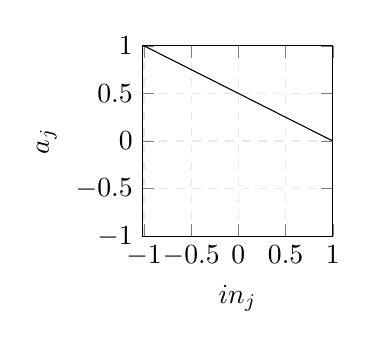
\begin{tikzpicture}
			\begin{axis}[
			width=4cm, height=4cm,     % size of the image
			grid = major,
			grid style={dashed, grey!30},
			xmax=1,        
			ymin=-1,
			ymax=1,
			axis background/.style={fill=white},
			ylabel=$a_{j}$,
			xlabel=$in_{j}$]
			
			\addplot[black]{-0.5*x+0.5};
		%	\addplot[black]{-2*x-1.5};
			\end{axis}
			\end{tikzpicture}
			\label{fig:sepplot1}
		}
		
\end{figure}

\paragraph{Applications}
The perceptron can be used as pattern associator to categorise an inputpattern to a class, competitive network. Also linear seperable data can be categorised.
It can be trained with the hebbian- or the delta-learning rule.(see also \eqref{sec:learning})

\begin{center}
	\begin{figure}[H]
		\centering
		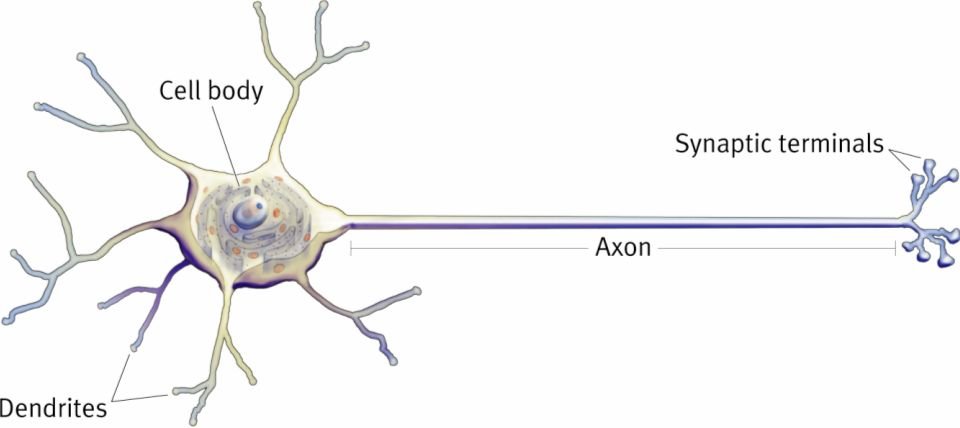
\includegraphics[width=0.8\textwidth,scale=1]{files/neuron.jpg}  
		\caption{A singlelayer perceptron \cite{PERSIN}.}
		\label{fig:neuron}
	\end{figure}
\end{center}

\subsection{Second generation}
The idea of the second generation of neural networks is born in the 90s. The firerate of a neuron encodes the transmitted signal. In this case now real values are used for in- and outputs.

\subsubsection{Multi layer perceptron (MLP)} \label{sec:mlp}
The multilayer perceptron was intruduced by Minsky and Papert in . It has an input-, an output- and
one or multiple hiddenlayers. In contrast to the singlelayerperceptron it can solve the xor-problem and other non-linear problems. It can be trained super- or unsupervised.


\subsubsection{Radial basis function} %Oder paragraph?


\subsubsection{Kohonen networks / Selforganizing maps (SOM)}
Kohonen-networks are inventioned by the finnish engineer Teuvo Kohonen in 1982. They have two layers. An inputlayer and a n-dimensional outputlayer.
Kohonen-networks usually don't have hidden layers.
The inputspace 
Data-mining, unsupervised learning, clusteranalysis, computergraphics. 

\subsection{Combination of networkmodels}

\subsubsection{MLP and SOM} %look at neuronale netze im klartext chapter 6.3

\subsection{Third generation}
In the third generation of artifical neural networks the signal is additionally encoded in time. These called spikes are

\subsubsection{Spiking neural networks}


%\subsection{Feed Forward}
\subsection{Recurrent}

%...
%\subsection{Pattern recognition}

%\subsection{Traveling salesman problem}

%\subsection{Aproximation of functions}
%...

\chapter{Optimization with evolutionary algorithms}
Optimization is widely used, for example in information technology, engineering,
economics, etc. Applications are the routing of circuits, the optimal usage of machinery,
the traveling-salesman-problem and much more. It is often difficult to create a mathematical
model of such optimization problems. Therefore in the last decades were developed methods who
uses principles of the evolution.
The simples method is the selection-method. In this model a dateset will be generated and randomly
changes, called mutations, are made. The best datasets, chosen by the best fitness, will be kept.
Each dateset is called an individual. A set of individuals is called a population. The individuals
of a population can be recombined. Mostly the best individuals are recombined with randomly chosen
ones. This method is more effective than the selection-method. This and other methods are  called
evolutionary algorithms. To use an evolutionary algorithm, the problem must not be in a defined form;
therefore it hasn't to be linear or differentiable. \\

In this project evolutionary algortihms are used to find the best 
(unsupervised) neural network to controll one creature. The idea is to use the amount of food a creature collect over a defined time as fitnessvalue.

\section{The creepy random search method or hill climber method}
The creepy random search method is a basic method of an evolutionary algorithm, developed by Ingo Rechenberg in 1973. % 1973 correct?? look at literaturesource in kinnebruck
Parameters of a system are randomly changed till a minimum or maximum of a targetfunction is reached. The value of the parameterchanges per iterationstep are limited. \\

\textbf{The main algorithm is:}

\fbox{
\begin{minipage}{15cm}
	\begin{enumerate} 
		\item Generate a randomly initialized chromosome.
		\item Change the chromosome parameter by limited random delta-values. 
		\item Prove if the chromosome has a better fitness than the old one and replace it. Otherwise forget the new chromosome.
		\item If the optimization-condition is reached abort, otherwise go to step 2.
	\end{enumerate}
\end{minipage}
} \\

The algorihm can be imagined as a blind hillclimber. The hillclimber makes a random step. If he gets higher, he makes the next step. Otherwise he takes back his last step and makes another random step. The big problem is, that this algorithm mostly converges in a local optimum. \\

\textbf{Reasons to use this kind of algorithm:}

\fbox{
	\begin{minipage}{15cm}
		\begin{itemize} 
			\item For many nonlinear problems there are no alternative solution approaches.
			\item Implementing this method is easy.
		\end{itemize}
	\end{minipage}
}   \\



\begin{center}
	\begin{figure}[H]
		\centering
		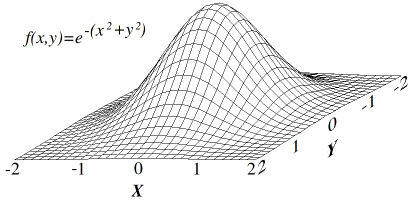
\includegraphics[width=0.6\textwidth,scale=1]{files/Hill_climb.png}  
		\caption{A convex function. Ideal for the hillclimbing method \cite{wiki-hill}.}
		\label{fig:hill}
	\end{figure}
\end{center}

\begin{center}
	\begin{figure}[H]
		\centering
		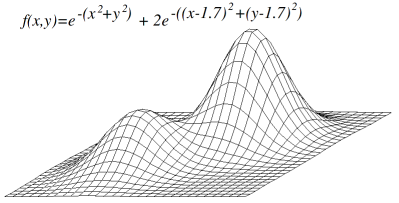
\includegraphics[width=0.6\textwidth,scale=1]{files/Local_maximum.png}  
		\caption{A function with two optima. Hillclimbing could end in the worse optimum if it starts at a bad coordinate. \cite{wiki-hill}.}
		\label{fig:hill2}
	\end{figure}
\end{center}


\subsection{Constraints} %Bedingungen und Nebenbedingungen
The main condition is the fitness-function. Second conditions
can be the

%\subsection{Efficency} %Optional chapter to test the efficency between mathematical methods and evolutionary methods. For example zero of a function.

\section{Variants of the creepy random search method}
In the main-method of the creepy random search you just accept better fitness values after an iteration-step and reject worse ones.
The problem is, that with this algorithm you will mostly get stuck on a local optimum, instead of finding the global one.
To solve this problem you should allow temporal low fitness-values. It should be possible to leave a local optimum to find a better one.
To realise this, there have been developed some extended versions of this method: \\

\fbox{
	\begin{minipage}{15cm}
		\begin{itemize} 
			\item A stagnation of the fitness is allowed by a specified probability (Simulated annealing)
			\item A stagnation of the fitness is allowed till a maximal deterioration. (Threshold accepting, deluge method)
		\end{itemize}
	\end{minipage}
} \\


\subsection{Simulated annealing}
Simulated annealing is a probabilistic optimization method.
It is inspired by the annealing of fluid materia to a solid aggregate states in metallurgy. While cooling down a material the thermodynamic free energy has to get as minimal as possible to get a clear crystalline structure. Therefore its suggested to cool down to material slowly for a better probability of getting a clear solid body.

Analog in optimization you start with a high temperature T, means a big delta, to make wide jumps in the problemphase-space. So jumps between more maxima are possible. At the beginning each chromosome has the same probability to get selected. With each iteration the temperature is reduced and the jumps are getting shorter. Selecting better chromosomes is now more probalistic.
Towards the end the algorithm commutes in a optimum and behaves like the standard hillclimbing-algorithm.

Slowly reducing the temperature increases the chance to find the global optimum. Cooling to fast leads to commuting early into a local optimum instead.

The following formula shows the probability of selecting a chromosome with lower fitness:

\begin{equation}
p(r) = \frac{1}{1+exp(-r/T)}
\end{equation} 

The probability to select a worse chromosome should be small.
At the beginning a big T tends to equalize the probability of all chromosomes. For $T \to \infty$ all chromosomes have the same chance to get selected. Lowering T gives good chromosomes priority. For T = 0.1

\subsection{Threshold accepting}

\section{Genetic algorithms - An artifical duck}

\section{}

\chapter{Other 'intelligent' algorithms}
In this chapter other intelligent algorithms are presented.
These algortihms are for comparing the neural network to simpler
methods.

\section{The greedy algorithm}

\subsection{Weaknesses}

\chapter{Evaluation}
\chapter{Related work}
\chapter{Conclusion}
\chapter{Future work}




\KOMAoptions{listof=leveldown}

\newpage

%=========================================LISTS=========================================

\listoffigures
\listoftables
\listofalgorithms
\lstlistoflistings

\newpage

%=========================================DICTIONARY====================================

%dictiary style
\bibliographystyle{./files/alphadin}
%dictionary source
\bibliography{./files/bibdb}

\end{document}
